\documentclass[12pt]{article}
\usepackage[utf8]{inputenc}
\usepackage[T1]{fontenc}
\usepackage[polish]{babel}
\usepackage{geometry}
\usepackage{tabularx}
\usepackage[table,xcdraw]{xcolor}
\usepackage{color}
\usepackage{subfig}
\usepackage{sidecap}
\usepackage{wrapfig}
\usepackage{float}
\usepackage{enumerate}
\usepackage{graphicx}
\usepackage{multirow}
\setlength{\parindent}{0pt}
\usepackage{hyperref}
\usepackage{titlesec}
\titlelabel{\thetitle.\quad}
\usepackage{amsmath}
\usepackage{anyfontsize}
\usepackage{indentfirst}
\usepackage{listings}
\usepackage{multicol}
\usepackage{pgfplots}
\usepackage{fancyhdr}

\definecolor{clr-background}{RGB}{255,255,255}
\definecolor{clr-text}{RGB}{0,0,0}
\definecolor{clr-string}{RGB}{163,21,21}
\definecolor{clr-namespace}{RGB}{0,0,0}
\definecolor{clr-preprocessor}{RGB}{128,128,128}
\definecolor{clr-keyword}{RGB}{0,0,255}
\definecolor{clr-type}{RGB}{59, 112, 230}
\definecolor{clr-variable}{RGB}{0,0,0}
\definecolor{clr-constant}{RGB}{111,0,138} % macro color
\definecolor{clr-comment}{RGB}{0,128,0}
\definecolor{mycolor}{rgb}{0.8,0.8,0.8}
\lstset{
  xleftmargin=20pt,
  xrightmargin=0pt,
  framexleftmargin=20pt,
  framexrightmargin=0pt,
  framexbottommargin=2pt,
  columns=flexible,
  keepspaces=true,
  showstringspaces=false,
  backgroundcolor=\color{clr-background},
  basicstyle=\color{clr-text}, % any text
  stringstyle=\color{clr-string},
  identifierstyle=\color{clr-variable}, % just about anything that isn't a directive, comment, string or known type
  commentstyle=\color{clr-comment},
  keywordstyle=\color{clr-type},
  tabsize=4,
  aboveskip=1em,
  belowskip=0em,
  frame=b,
  rulecolor=\color{mycolor},
  numbers=left,
  numbersep=10pt,
  numberstyle={\fontsize{9pt}{11pt}\selectfont\color{gray}},
}




\newgeometry{tmargin=1.8cm,bmargin=1.8cm,lmargin =1.8cm,rmargin=1.8cm}
\pagestyle{fancy}
\fancyhf{}
\rhead{\textit{Jakub Kusz}}
\lhead{\textit{ MiniMax z alfa-beta cięciami }}
\cfoot{ \thepage}

\begin{document}
    \begin{titlepage}
\begin{figure}
	\centering
	\includegraphics[width=18cm]{//home/kubus/Obrazy/logo-Pwr.png}
	
	\label{fig:pwr}
\end{figure}
	\begin{center}
		\huge Wydział Elektroniki, Fotoniki i Mikrosystemów \\ 
		\vspace{40pt}
		\huge PAMSI  \\
	\end{center}
	\vspace{60pt}
	\hrule
	\vspace{1pt}
	\hrule
	\begin{center}
		{\fontsize{40}{50}\selectfont Sprawozdanie nr 1\\ }
		\vspace{10pt}
		{\fontsize{25}{25}\selectfont Projekt - marzec  }
	\end{center}
	\hrule
	\vspace{1pt}
	\hrule
	\begin{flushright}
		\vspace{65pt}
		\textit{\Large Prowadzący:}\\
		
		\Large dr hab. inż. Andrzej Rusiecki\\
		\vspace{10pt}
		\textit{\Large Wykonał:}\\
		
		\Large Jakub Kusz \\
	
	\end{flushright}
	\vspace{100pt}
	\begin{center}
		\large Wrocław, \today r.
	\end{center}
\end{titlepage}



    \tableofcontents
    \newpage
    \section{Cel ćwiczenia}
        Celem ćwiczenia jest zaimplementowanie algorytmu MiniMax z alfa-beta cięciami w grze kółko i krzyżyk.
        Użytkownikowi dano możliwość wyboru poziomu trudności (głębokość algorytmu) i wielkości planszy.
    \section{Wstęp}
        \subsection{MiniMax}
            MinimMax jest algorytmem służącym do  minimalizowania maksymalnych możliwych strat. Alternatywnie można je traktować 
            jako maksymalizację minimalnego zysku. Wywodzi się to z teorii gry o sumie zerowej, obejmujących oba przypadki, 
            zarówno ten, gdzie gracze wykonują ruchy naprzemiennie, jak i ten, gdzie wykonują ruchy jednocześnie. 
            Zostało to również rozszerzone na bardziej skomplikowane gry i ogólne podejmowanie decyzji w obecności niepewności. 
            \subsubsection{Zasada działania}
                Najprostszym sposobem przedstawiania zasady działania algorytmu MiniMax jest ukazanie jego pracy na przykładzie.
                Na rysunku \ref{fig: drzewo}, pokazujemy wyniki uzyskane przez gracza x w każdym momencie gry. W bazie, na pierwszym poziomie, decyzję podejmuje przeciwnik. Z tego powodu podane są scenariusze, w których gracz może stracić -10 lub wygrać 5.
                Na drugim poziomie zależy to od gracza x, więc zmaksymalizuje on swój zysk. Pomiędzy stratą 10 a wygraną 1 wygrasz 1. Podobnie, jeśli wygrasz 5 lub 7, wygrasz 7.
                Potem znowu kolej na przeciwnika, więc zostaną podane scenariusze, w których gracz x ma najgorszy wynik, -3 i 4, w zależności od przypadku. Wreszcie, pomiędzy przegraną 3 a wygraną 4, gracz x podejmie decyzję, która pozwoli temu drugiemu.

                \begin{figure}[H]
                    \centering
                    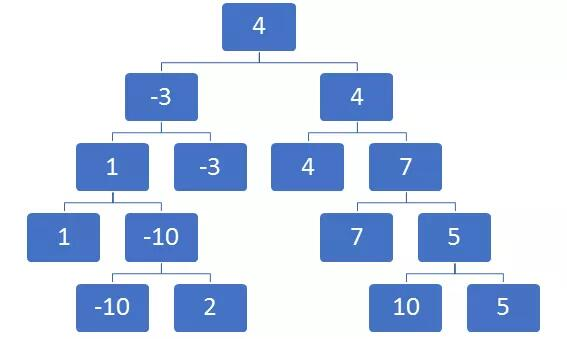
\includegraphics[width = 15cm]{drzewo.jpeg}
                    \caption{Drzewo przeszukiwań}
                    \label{fig: drzewo}
                    
                \end{figure}

            \subsection{Alfa-beta cięcia}
            Korzyść płynąca z algorytmu alfa-beta leży w fakcie, że niektóre gałęzie drzewa przeszukiwania mogą zostać odcięte. Czas przeszukiwania ograniczony zostaje do przeszukania najbardziej obiecujących poddrzew, w związku z czym możemy zejść głębiej w tym samym czasie. Tak samo jak klasyczny min-max, algorytm należy do algorytmów wykorzystujących metody podziału i ograniczeń. Współczynnik rozgałęzienia jest dwukrotnie mniejszy niż w klasycznym  MiniMax. Algorytm staje się wydajniejszy, gdy węzły rozwiązywane są układane w porządku optymalnym lub jemu bliskim.
            
    \section{Implementacja}
        
        Z powodu ograniczeń związanych ze sprzętem nie jesteśmy w stanie rozwinąć całego drzewa od początku do końca, wiec algorytm MiniMax działa do 
        określonej głębokości, na której  następuje ocena pozycji za pomocą przeznaczonej do tego funkcji.Implementacja całej gry w języku C++ została umieszczona \href{https://github.com/PartyKusZ/PAMSI/tree/main/projekt_3-czerwiec}{\textbf{tutaj}}.
        \subsection{Ocena pozycji}
            Do oceny pozycji po osiągnięciu danej głębokości została napisana metoda  evaluate\_position(), która ocenia 
            pozycje na podstawie ilości kółek/krzyżyków z rzędu.
            \begin{lstlisting}[language=C++, caption=evaluate\_position()]
    void t_game :: evaluate_position(){
        int tmp;
        for(int i = 0; i < number_of_fields; ++i){
            tmp = 0;
            for(int j = 0; j < number_of_fields; ++j){
                if(gameborad_table[i][j] == 'o'){
                    tmp++;
                }else if(gameborad_table[i][j] == 'x'){
                    tmp = 0;
                    break;
                }
            }
            if(tmp){
                position_rating += pow(10,tmp);
            }
        }
    
        for(int i = 0; i < number_of_fields; ++i){
            tmp = 0;
            for(int j = 0; j < number_of_fields; ++j){
                if(gameborad_table[j][i] == 'o'){
                    tmp++;
                }else if(gameborad_table[j][i] == 'x'){
                    tmp = 0;
                    break;
                }
            }
            if(tmp){
                position_rating += pow(10,tmp);
            }
        }
        tmp = 0;
        for(int j = 0; j < number_of_fields; ++j){
            tmp = 0;
                if(gameborad_table[j][j] == 'o'){
                    tmp++;
                }else if(gameborad_table[j][j] == 'x'){
                    tmp = 0;
                    break;
                }
                if(tmp){
                    position_rating += pow(10,tmp);
                }
            }
            
        tmp = 0;
        for(int i = 0, j = number_of_fields - 1; i < number_of_fields; ++i, --j){
            tmp = 0;
                if(gameborad_table[i][j] == 'o'){
                    tmp++;
                }else if(gameborad_table[i][j] == 'x'){
                    tmp = 0;
                    break;
                }
                if(tmp){
                    position_rating += pow(10,tmp);
                }
            }
            
       
    }
                
            \end{lstlisting}
                
    

        \subsection{MiniMax z alfa-beta cięciami}
            Metoda znajdująca najlepsze zagranie: Na początku sprawdzane jest czy któryś z zawodników wygrał, jeśli tak to zwracamy maksymalnie/minimalnie duże oceny pozycji i funkcja się kończy.
            Jeśli nikt nie wygrał, to po osiągnięciu danej głębokości następuje ocena pozycji i zwrócenie jej wartości. Jeśli nie osiągnęliśmy jeszcze zadanej głębokości,
            algorytm wykonuje naprzemiennie ruchy graczy i wywołuje się rekurencyjnie. Po osiągnięciu ostatniego wywołania funkcji do działania przystępują alfa-beta cięcia.
            

            \begin{lstlisting}[language=C++, caption=minimax\_alpha\_beta()]
    int t_game :: minimax_alpha_beta(who_start current_player,  int depth, long int a, long int b){
    this->check_win();
    if(winner != who_start::draw){
        if(current_player == who_start :: ai){
            return INT32_MAX;
        }else{
            return INT32_MIN;
        }
    }
    if(this->is_finish() || depth == 0){
        if(current_player == who_start :: ai){
             this->evaluate_position();
             return position_rating;
        }else{
             this->evaluate_position();
             return -position_rating;
        }
    }
   long int best_score;
    if(current_player == who_start :: human){
        current_player = who_start :: ai;
        best_score = INT64_MIN;
    }else{
        current_player = who_start :: human;
        best_score = INT64_MAX;
    }
    int tmp;
    for(int i = 0; i < number_of_fields; ++i){
        for(int j = 0; j < number_of_fields; ++j){
            if(gameborad_table[i][j] == '_'){
                if(current_player == who_start :: ai){
                    gameborad_table[i][j] = 'o';
                    tmp = this->minimax_alpha_beta(current_player, depth-1, a, b);
                    if(best_score < tmp){
                        best_score = tmp;
                    }
                    if(a < best_score){
                        a = best_score;
                    }
                    gameborad_table[i][j] = '_';
                    if(a >= b){
                        return best_score;
                    }
                }else{
                    gameborad_table[i][j] = 'x';
                    tmp = this->minimax_alpha_beta(current_player, depth-1, a, b);
                    if(best_score > tmp){
                        best_score = tmp;
                    }
                    if(a > best_score){
                        a = best_score;
                    }
                    gameborad_table[i][j] = '_';
                    if(a >= b){
                        return best_score;
                    }
                }
            }
        } 
    }
    return best_score;
}
            \end{lstlisting}
    \subsection{Ustalenie współrzędnych najlepszego posunięcia}
    Do wyboru współrzędnych dla najlepszego posunięcia została napisana poniższa metoda:
    \begin{lstlisting}[language=C++, caption=best\_ai\_move()]
    void t_game ::  best_ai_move(int depth){

    long int best_score = INT64_MIN;
    int tmp;
    int set_i;
    int set_j;
    for(int i = 0; i < number_of_fields; ++i){
        for(int j = 0; j < number_of_fields; ++j){
            if(gameborad_table[i][j] == '_'){
                gameborad_table[i][j] = 'o';
                tmp = minimax_alpha_beta(who_start :: ai, depth, INT64_MIN, INT64_MAX);

                gameborad_table[i][j] = '_';
                if(tmp > best_score){
                    best_score = tmp;
                    set_i = i;
                    set_j = j;
                }
            }
        }
    }
    if(set_i < number_of_fields && set_j < number_of_fields)
        gameborad_table[set_i][set_j] = 'o';
}

\end{lstlisting}

\section{Środowisko graficzne - SFML}
W celu przyjemnego przedstawienia rozgrywki została wykorzystana biblioteka graficzna SFML.
Cechuje się ona łatwością użycia, nieskomplikowanym procesem konfiguracyjnym i dobrą wydajnością.
\subsection{Obliczanie odstępów między liniami stanowiącymi planszę}

    Aby obliczyć odstępy między liniami stanowiącymi planszę rozmiar okna został podzielony przez 
    ilość pól w kolumnie. Znając rozmiar pola łatwo można narysować linię stanowiące planszę.

    \begin{lstlisting}[language=C++, caption=set\_gameboad\_table()]
    
    void t_gameboard :: set_gameboad_table( sf :: Vector2i xy){
        player = who_start :: ai;
        xy.x = xy.x / filed_size;
        xy.y = xy.y / filed_size;
        if((xy.x < number_of_fields )&& (xy.y < number_of_fields)){
            if(gameborad_table[xy.x][xy.y] == '_'){
                if(player == who_start :: ai){
                    if(++move_counter % 2 == 0){
                        gameborad_table[xy.x][xy.y] = 'x';
                    }else{
                        gameborad_table[xy.x][xy.y] = 'x';
                    }

                }
                if(player == who_start :: human){
                    if(++move_counter % 2 == 1){
                        gameborad_table[xy.x][xy.y] = 'x';
                    }else{
                        gameborad_table[xy.x][xy.y] = 'x';
                    }

                }
            }
        }
        
    
}


    \end{lstlisting}
    

    \subsection{Rysowanie planszy, kółek, krzyżyków i zwycięstwa}

        Poniższa wirtualna z biblioteki SFML została wykorzystana do rysowania całego stanu gry:

    \begin{lstlisting}[language=C++, caption=draw()]
        
void t_game :: draw(sf::RenderTarget& target, sf::RenderStates states)const{
    
     t_circe circle;
     t_cross cross;
     int circle_win = 0;
     int cross_win = 0;
     circle.setCharacterSize(filed_size);
     cross.setCharacterSize(filed_size);
     for(int i = 0; i < lines.size(); ++i){
         target.draw(lines[i],states);
     }
     for(int i = 0; i < number_of_fields; ++i){
         for(int j = 0; j < number_of_fields; ++j){
             
            if(gameborad_table[i][j] == 'x'){
                cross.set_position(i * filed_size, j * filed_size);
                target.draw(cross,states);
            }
            if(gameborad_table[i][j] == 'o'){
                circle.set_position(i * filed_size , j * filed_size);
                target.draw(circle,states);
            }
         }
     }
     int circles;
     int crosses;
     circle.setColor(sf :: Color :: Green);
     cross.setColor(sf :: Color :: Green);
     for(int i = 0; i < number_of_fields; ++i){
         for(int j = 0; j < number_of_fields; ++j){
             if(gameborad_table[i][j] == 'o'){
                circles++;
            }
            if(gameborad_table[i][j] == 'x'){
                crosses++;
            }
         }
         if(circles == number_of_fields){
             for(int j = 0; j < number_of_fields; ++j){
                circle.set_position(i * filed_size , j * filed_size);
                target.draw(circle,states);
             }
             return;
        }
        if(crosses == number_of_fields){
            for(int j = 0; j < number_of_fields; ++j){
                cross.set_position(i * filed_size , j * filed_size);
                target.draw(cross,states);
             }
             return;

        }
        circles = 0;
        crosses = 0;
     }  

     for(int i = 0; i < number_of_fields; ++i){
         for(int j = 0; j < number_of_fields; ++j){
             if(gameborad_table[j][i] == 'o'){
                circles++;
            }
            if(gameborad_table[j][i] == 'x'){
                crosses++;
            }
         }
         if(circles == number_of_fields){
             for(int j = 0; j < number_of_fields; ++j){
                circle.set_position(j * filed_size , i * filed_size);
                target.draw(circle,states);
             }
             return;

        }
        if(crosses == number_of_fields){
            for(int j = 0; j < number_of_fields; ++j){
                cross.set_position(j * filed_size , i * filed_size);
                target.draw(cross,states);
             }
             return;

        }
        circles = 0;
        crosses = 0;
     }  


     for(int j = 0; j < number_of_fields; ++j){
             if(gameborad_table[j][j] == 'o'){
                circles++;
            }
            if(gameborad_table[j][j] == 'x'){
                crosses++;
            }
         }
         if(circles == number_of_fields){
             for(int j = 0; j < number_of_fields; ++j){
                circle.set_position(j * filed_size , j * filed_size);
                target.draw(circle,states);
             }
             return;

        }
        if(crosses == number_of_fields){
            for(int j = 0; j < number_of_fields; ++j){
                cross.set_position(j * filed_size , j * filed_size);
                target.draw(cross,states);
             }
             return;

        }
        circles = 0;
        crosses = 0;

        for(int i = 0, j = number_of_fields - 1; i < number_of_fields; ++i, --j){
             if(gameborad_table[i][j] == 'o'){
                circles++;
            }
            if(gameborad_table[i][j] == 'x'){
                crosses++;
            }
         }
         if(circles == number_of_fields){
             for(int i = 0, j = number_of_fields - 1; i < number_of_fields; ++i, --j){
                circle.set_position(i * filed_size , j * filed_size);
                target.draw(circle,states);
             }
             return;

        }
        if(crosses == number_of_fields){
            for(int i = 0, j = number_of_fields - 1; i < number_of_fields; ++i, --j){
                cross.set_position(i * filed_size , j * filed_size);
                target.draw(cross,states);
             }
             return;

        }
        circles = 0;
        crosses = 0;
}

    \end{lstlisting}
                

\section{Testy}
    Gra została przetestowana pod względem poprawności działania i wydajności. 
        \subsection{Poprawność działania}
            Po rozegraniu wielu gier stwierdzono, że algorytm działa poprawnie, stara się wyszukiwać najlepsze ruchy,
            blokuje możliwości wygrania przez człowieka, najlepszą możliwością jest remis.
            Z obserwacji wynika, że już przy głębokości 1 nie człowiek nie jest w stanie wygrać z komputerem.
        \subsection{Wydajność}

        Aby gra przebiegała sprawie, dla danych rozmiarów planszy, zostały arbitralnie przydzielone maksymalne głębokości algorytmu:
        \begin{table}[H]
            \centering
            \caption{Zawierajaca czasy obliczania pierwszego ruchuchu algorytmu MiniMax dla danej wielkości planszy}
            \begin{tabular}{|c|c|c|}
            \hline
            Wielkość planszy & Głebokość maksymalna                                                                                           & Czas oczekiwania na pierwszy ruch {[}ms{]} \\ \hline
            3                & \begin{tabular}[c]{@{}c@{}}dowolna, algorytm jest w stanie \\ szybko rozwinąć grę do samego końca\end{tabular} & 90                                         \\ \hline
            4                & 5                                                                                                              & 1523                                       \\ \hline
            5                & 4                                                                                                              & 1816                                       \\ \hline
            6                & 3                                                                                                              & 480                                        \\ \hline
            7                & 3                                                                                                              & 1891                                       \\ \hline
            8                & 2                                                                                                              & 114                                        \\ \hline
            9                & 2                                                                                                              & 271                                        \\ \hline
            10               & 2                                                                                                              & 589                                        \\ \hline
            \end{tabular}
            \end{table}
           Zastosowanie większych głębokości dla danych rozmiarów planszy wiązało się z bardzo długim oczekiwaniem na ruch komputera w początkowej fazie gry. Wraz z każdym ruchem czas oczekiwania na odpowiedź komputera zmniejsza się. 
            \section{Wnioski}
            \begin{itemize}
                \item Algorytm MiniMax wraz z alfa-beta cięciami doskonale nadaje się do symulacji gracze w grze o sumie zerowej;
                \item Dzięki zastosowaniu alfa-beta cięć algorytm znacząco skraca czas działania, dzięki odcinaniu gałęzi niemających znaczenia dla rozwoju gry,
                \item Algorytm nawet na głębokości 1 jest w stanie skutecznie powstrzymać zwycięstwo człowieka, pozwalając maksymalnie na remis.
                \item Ważne jest aby dopasować głębokość do wielkości planszy. Zbyt duża głębokość znacząco wydłuża działanie programu.
                \item SFLM jest potężnym narzędziem do tworzenia GUI, niestety brakuje w tej bibliotece prostej obsługi przycisków i obsługi pól tekstowych przez co poziom trudności i wymiar planszy należy podać w terminalu.
            \end{itemize}
\end{document}
